\documentclass[a4paper, 10pt]{article}
\usepackage{common}
\usepackage{enumitem}
\newenvironment{QandA}{
    \begin{enumerate}\bfseries}
    {\end{enumerate}
}
\newenvironment{answered}{\par\normalfont}{}
\pagestyle{empty}

\begin{document}
    
% Carátula
\title{
    \faIcon[regular]{gem}\\
    Programación Concurrente\\
    \large Preguntas de final
}

\author{Ramiro Martínez D'Elía}
\date{2021}
\maketitle

\noindent%
\begin{QandA}
\item Defina programa concurrente, programa paralelo y programa distribuido.
\begin{answered}
    \emph{Apunte I: sección 1.1, Apunte II: sección 1.1 y Apunte IV: 1.1}
\end{answered}

%========================================================================

\item Responda
\begin{enumerate}[label=\alph*)]
\item ¿A qué se denomina propiedad del programa? ¿Qué son las propiedades de seguridad y vida? Ejemplificar.
\begin{answered}
    \emph{Apunte I: sección 1.1, Apunte II: sección 1.1 y Apunte IV: 1.1}
\end{answered}
\item Defina fairness. Relacionar dicho concepto con las políticas de scheduling.
\begin{answered}
    \emph{Apunte I: sección 1.7}
\end{answered}
\item Describa los distintos tipos de fairness
\begin{answered}
    \emph{Apunte I: sección 1.8}
\end{answered}
\item ¿Cuáles son las propiedades que debe cumplir un protocolo de E/S a una sección crítica?
\begin{answered}
    \emph{Apunte II: sección 1.2}
\end{answered}
\item Cuáles son los defectos que presenta la sincronización por busy waiting? Diferencie esta situación respecto de los semáforos.
\begin{answered}
    \emph{Apunte II: sección 2.3}
\end{answered}
\item Explique la semántica de la instrucción de grano grueso  AWAIT y su relación con las instrucciones Test \& Set o Fetch \& Add.
\begin{answered}
    \emph{Apunte I: sección 1.6}
\end{answered}
\end{enumerate}

%===================================================================================================

\item Definir el problema general de alocación de recursos y su resolución mediante una política SJN. ¿Minimiza el tiempo promedio de espera? ¿Es fair? Si no lo es, plantee una alternativa que lo sea.
\begin{answered}
    \emph{Apunte II: sección 3.5.2}
\end{answered}

%===================================================================================================

\item ¿En qué consiste la técnica de passing the baton? Aplicar este concepto a la resolución del problema de lectores y escritores.
\begin{answered}
    \emph{Apunte II: sección 3.5 y 3.5.1}
\end{answered}

%===================================================================================================

\item Explique el concepto de broadcast y sus dificultades de implementación en un ambiente distribuido, con pasaje de mensajes sincrónico y asincrónico.
\begin{answered}
\emph{Sobre primitiva broadcast $\rightarrow$ Apunte III: sección 2.1.4}

En un ambiente con memoria compartida, este tipo de primitivas es más sencilla de implementar.

En ambientes distribuidos, al no haber variables compartidas, se debe utilizar pasaje de mensajes. Esto, supone ciertas dificultades para cada caso.

Con pasaje de mensajes asincrónicos (PMA), podemos plantear los siguientes escenarios de implementación:

\underline{Utilizar un único canal}

El emisor deberá enviar tantos mensajes, como receptores existan. Este escenario evita demoras innecesarias, en el envío de mensajes, ya que \lstinline{send} no es bloqueante.

\underline{Un canal por proceso}

El  emisor  deberá  enviar  el  mensaje  por  tantos  canales,  como  receptores  existan.  Con  este  escenario, tenemos demoras innecesarias: un proceso listo debe esperar a que el emisor itere sobre su canal.

Con pasaje de mensajes sincrónicos (PMS), los canales son punto a punto. Por este motivo, solo podemos llevar a cabo la implementación ``un canal por proceso'' planteada en PMA. Aunque, en este caso, resulte aún más ineficiente ya que \lstinline{send} demora.

\end{answered}

%====================================================================================================

\item Sobre exclusión mutua selectiva

\begin{enumerate}[label=\alph*)]
\item ¿Por qué el problema de los filósofos es de exclusión mutua selectiva? Si en lugar de 5 filósofos fueran 3, ¿el problema seguiría siendo de exclusión mutua selectiva? ¿Por qué?
\begin{answered}
    \emph{Apunte II: sección 3.4.1}
\end{answered}
\item El problema de los filósofos resuelto de forma centralizada y sin posiciones fijas ¿es de exclusión mutua selectiva? ¿Por qué?
\begin{answered}
    \emph{Apunte II: sección 3.4.1}
\end{answered}
\item El problema de los lectores-escritores es de exclusión mutua selectiva? ¿Porque?
\begin{answered}
    \emph{Apunte II: sección 3.4.2}
\end{answered}
\item Si en el problema de los lectores-escritores se acepta sólo 1 escritor  o 1 lector en la BD, ¿tenemos un problema de exclusión mutua selectiva?  ¿Por qué?
\begin{answered}
    \emph{Apunte II: sección 3.4.2}
\end{answered}
\end{enumerate}

%=====================================================================================================

\item Sea el problema en el cual N procesos poseen inicialmente cada uno un valor V, y el objetivo es que todos conozcan cual es el máximo y cuál es el mínimo de todos los valores.

\begin{enumerate}[label=\alph*)]
\item Plantee conceptualmente posibles soluciones con las siguientes arquitecturas de red: Centralizada, simétrica y anillo circular. No implementar.
\begin{answered}
    \emph{Apunte III: sección 2.1}
\end{answered}
\item Analice las soluciones anteriores desde el punto de vista del número de mensajes y la performance global del sistema.
\begin{answered}
    \emph{Apunte II: sección 2.1.4}
\end{answered}
\end{enumerate}

%======================================================================================================

\item Defina el concepto de granularidad. ¿Qué relación existe entre la granularidad de programas y de procesadores?
\begin{answered}
    \emph{Apunte IV: sección 1.6}
\end{answered}

%========================================================================================================

\item Dado el siguiente programa concurrente con memoria compartida, y suponiendo que todas las variables están inicializadas en 0 al empezar el programa, y que las instrucciones no son atómicas. Para cada una de las opciones indique verdadero o falso. En caso de ser verdadero indique el camino de ejecución para llegar a ese valor y de ser falso justifique claramente su respuesta.

\begin{multicols}{3}
\begin{lstlisting}
P1::            
If ( x == 0 ) then
    Y = 4*x+2;
    X = y+2+x;
\end{lstlisting}
\columnbreak
\begin{lstlisting}
P2::            
If ( x > 0 ) then
    X = X + 1;
\end{lstlisting}
\columnbreak
\begin{lstlisting}
P3::            
X = x*8+x*2+1;
\end{lstlisting}
\end{multicols}

\begin{enumerate}[label=\alph*)]
\item El valor de x al terminar el programa es 9.
\begin{answered}
\emph{Instrucciones no atómicas $\rightarrow$ los bloques IF pueden ser interrumpidos\\} 
Verdadero para la siguiente historia:\\
$P1_2 \rightarrow P2 \rightarrow P3 (x=1) \rightarrow P1_3 (y=2) \rightarrow P1_4 (x=9)$
\end{answered}
\item El valor de x al terminar el programa es 6.
\begin{answered}
Verdadero para la siguiente historia:\\
$P1_2 \rightarrow P1_3 (y=2) \rightarrow P3 (x=1) \rightarrow P1_4 (x=5) \rightarrow P2 (x=6)$
\end{answered}
\item El valor de x al terminar el programa es 11.
\begin{answered}
Falso: la única forma de que ocurra es que $x=1$ cuando se ejecute P3. Esto no puede darse, ya que P2 nunca podría incrementar con $x=0$ y P1 escribe valores mayores sobre $x$.
\end{answered}
\item Y, siempre termina con alguno de los siguientes valores: 10 o 6 o 2 o 0.
\begin{answered}
\begin{itemize}
\item $y=10$ con $P1_2 \rightarrow P3 (x=1) \rightarrow P2 (x=2) \rightarrow P1_3 (y=10) \rightarrow P1_4 (x=8)$
\item $y=6$ con $P1_2 \rightarrow P2 \rightarrow P3 (x=1) \rightarrow P1_3 (y=6) \rightarrow P1_4 (x=9)$
\item $y=2$ con cualquier historia que inicie con $P1_2 \rightarrow P1_3$. Una vez seteado $y$, ningún otra instrucción la modifica.
\item $y=0$ con cualquier historia que inicie con $P3$. Ya que $x=1$ invalidará el if de P1.
\end{itemize}
\end{answered}
\end{enumerate}

%=====================================================================================================

\item ¿En qué consiste la comunicación guardada (introducida por CSP) y cuál es su utilidad?
\begin{answered}
    \emph{Apunte III: sección 3.1}
\end{answered}

%=====================================================================================================

\item ¿Cuál es la utilidad de la técnica de passing the baton? ¿Qué relación encuentra con la técnica de passing the condition?
\begin{answered}
    \emph{Apunte II: sección 3.5}
\end{answered}

%=====================================================================================================

\item Explique sintéticamente los 7 paradigmas de interacción entre procesos en programación distribuida. Ejemplifique.
\begin{answered}
    \emph{Apunte III: capitulo 5}
\end{answered}

%=====================================================================================================

\item Responder sobre programación paralela
\begin{enumerate}
    \item ¿Cuál es el objetivo de la programación paralela?
    \begin{answered}
        \emph{Apunte IV: sección 1.1}
    \end{answered}
    \item Defina las métricas de speedup y eficiencia. ¿Cuál es el significado de cada una de ellas (que miden)? ¿Cuál es el rango de valores para cada una?
    \begin{answered}
        \emph{Apunte IV: sección 1.2 y sección 1.3}
    \end{answered}
    \item ¿En qué consiste la ley de Amdahl?
    \begin{answered}
        \emph{Apunte IV: sección 1.5}
    \end{answered}
\end{enumerate}

%=======================================================================================================

\item Sea el problema de ordenar de menor a mayor un arreglo de A[1..n] 

\begin{enumerate}[labelindent=0pt, align=left, leftmargin=0pt]
\item Escriba un programa donde dos procesos (cada uno con n/2 valores) realicen la operación en paralelo mediante una serie de intercambios. 
\begin{answered}
En la siguiente implementación, el proceso P1 se queda con los números más chicos en su porción del arreglo. Mientras que, el proceso P2 con los números más grandes.
\begin{lstlisting}[multicols=2]
Process P1
const mayor = n/2;
int nuevo,
    a1[1:n/2];

# ordenar a1 de forma ascendente

P2 ! (a1[mayor]); # (1)
P2 ? (nuevo);

do (true) a1[mayor] > nuevo ->
    # reordenar a1:
    # decartando a1[mayor]
    P2 ! (a1[mayor]);
    P2 ? (nuevo)
od
end;
Process P2
const menor = 1;
int nuevo,
    a1[1:n/2];

# ordenar a1 de forma ascendente

P1 ? (nuevo);
P1 ! (a1[menor]); # (2)

do (true) a1[menor] < nuevo ->
    # reordenar a1:
    # descartando a1[menor]
    P1 ? (nuevo);
    P1 ! (a2[menor]);
od
end;
\end{lstlisting}
\end{answered}
\item ¿Cuántos mensajes intercambian en el mejor de los casos? ¿Y en el peor de los casos? 
\begin{answered}
\textbf{Mejor de los casos} $\rightarrow$ 2 mensajes totales (uno cada proceso).
\\
La lista ya se encuentra ordenada. Solo se envían los mensajes (1) y (2). Los valores enviados no satifacen la guarda del do, causando su finalización.
\\
\textbf{Peor de los casos} $\rightarrow n$ mensajes totales.
\\
La lista está ordenada de mayor a menor, todos los valores son intercambiados ($n/2$ cada proceso).
\end{answered}
\item Implemente una solución general a $k$ procesos, con $n/k$ valores cada uno (\emph{odd-even/exchange sort})
\begin{answered}
\begin{lstlisting}
Process worker[i = 1..k]

int largest = n/k, smallest = 1,
    a[1:k], dato;

# Ordeno la porcion del arreglo
# del proceso actual.

for(ronda = 1; ronda <= k; ronda++)

    if (i mod 2 == ronda mod 2)
        # Misma paridad (proceso+ronda par o proceso+ronda impar)
        if (i != k)
            proc[i+1]!(a[largest]);
            proc[i+1]?(dato);

            while (a[largest] > dato)
                # Inserto dato ordenado, pisando a[largest].
                proc[i+1]!(a[largest]);
                proc[i+1]?(dato);
            end;
        end;
    else
        if (i != 1)
            proc[i-1]?(dato);
            proc[i-1]!(a[smallest]);

            while (a[smallest] < dato)
                # inserto dato ordenado, pisando a[smallest].
                proc[i-1]?(dato);
                proc[i-1]!(a[smallest]);
            end;
        end;
    end;
end;
End.
\end{lstlisting}
\end{answered}
\item ¿Cuántos mensajes se intercambian en (c) en el mejor caso? ¿Y en el peor de los casos?
\begin{answered}
    \textbf{Peor caso} $\rightarrow$ la lista está ordenada de forma descendente (mayor a menor). En cuyo caso, los procesos deben intercambiar todos sus valores (en cada ronda). Por ejemplo, con $n=8$ y $k=4$:
    \\
    $\#MensajesRondasImpares = \#NumsPorProceso * \#ProcesosActivos * \#Rondas$
    \\
    $\#MensajesRondasImpares = n/k * k * k/2 = 8/4 * 4 * 4/2 = 2 * 4 * 2 = 16$ 
    \\
    $\#MensajesRondasPares = \#NumsPorProceso * \#ProcesosActivos - 2 * \#Rondas$
    \\
    $\#MensajesRondasPares = n/k * k-2 * k/2 = 8/4 * 4-2 * 4/2 = 2 * 2 * 2 = 8$ 
    \\
    $\#Mensajes = \#MensajesRondasPares + \#MensajesRondasImpares = 8 + 16 = 24$
    \\
    \textbf{Mejor caso} $\rightarrow$ la lista está ordenada de forma ascendente (menor a mayor). Seguimos la misma lógica, del caso anterior, pero entendiendo que cada proceso solo intercambia 1 único valor por ronda. Por ejemplo, con $n=8$ y $k=4$:
    \\
    $\#MensajesRondasImpares = 1 * k * k/2 = 1 * 4 * 4/2 = 1 * 4 * 2 = 8$
    \\
    $\#MensajesRondasPares = 1 * k-2 * k/2 = 1 * 4-2 * 4/2 = 1 * 2 * 2 = 4$
    \\
    $\#Mensajes = \#MensajesRondasPares + \#MensajesRondasImpares = 8 + 4 = 12$
\end{answered}

\item ¿Cómo modificaría el algoritmo del punto (c) para que termine tan rápido como el arreglo este ordenado? ¿Esto agrega overhead de mensajes? De ser así, ¿Cuánto?
\begin{answered}
Se podría implementar un proceso coordinador para lograr la siguiente interacción:. Al final de cada ronda, los procesos le indican al coordinador si efectuaron cambios en su colección de números
\begin{itemize}
    \item Los procesos, al final de cada ronda, le notifican al coordinador si efectuaron cambios en su colección de números.
    \item Si el coordinador, para una ronda, no recibe ninguna notificación de cambios entonces; da por concluido el trabajo y notifica a los procesos.
\end{itemize}
Esto, claramente, agrega un overhead en el pasaje de mensajes. Ya que, luego de cada ronda el coordinador recibirá $k$ mensajes (1 por proceso) y envará otros $k$ mensajes (1 a cada proceso). Dando un overhead, total, de $2k$
\end{answered}
\item ¿Considere que es más adecuado para este caso, si pasaje de mensajes sincrónico o asincrónico? Justifique.
\begin{answered}
PMS resulta la opción más adecuada ya que los procesos deben sincronizar de a pares. El comportamiento bloqueante del send/receive produce, de forma implícita, una barrera simética.
\\
En caso de emplear PMA, deberíamos implementar de forma explicita la barrera simétrica.
\end{answered}
\end{enumerate}

%=====================================================================================================================

\item Suponga que quiere ordenar N números enteros utilizando pasaje de mensajes con el siguiente algoritmo (odd/even Exchange sort): Hay  n procesos P [1: n], con n par. Cada proceso ejecuta una serie de rondas. En las rondas impares, los procesos con número impar P[impar] intercambian valores con P [impar +1] si los números están desordenados. En las rondas pares, los procesos con numero par P[par] intercambian valores con P [par +1] si los números están desordenados (P [1] y P[n] no hacen nada en las rondas pares).
\begin{enumerate}
    \item Determine cuantas rondas deben ejecutarse en el peor caso para ordenar los números.
    \begin{answered}
        \textbf{Peor caso} $\rightarrow$ la lista está ordenada de forma descendente (mayor a menor).
        \\
        En este caso, el algoritmo requerirá de $n$ rondas. Ya que requiere, enviar el máximo valor $n$ posiciones hacia delante. Con el valor mínimo, ocurre lo mismo; es necesario moverlo $n$ posiciones hacia atrás. Ambos desplazamientos se dan en simultáneo.
    \end{answered}
    \item ¿Considere que es más adecuado para este caso, si pasaje de mensajes sincrónico o asincrónico? Justifique.
    \begin{answered}
        \emph{Misma respuesta que en el caso general para $k$ procesos.}
    \end{answered}
\end{enumerate}

\item Dado el siguiente programa concurrente con memoria compartida, tenga en cuenta que las instrucciones no son atómicas:
\\
\begin{lstlisting}
x:=4; y:=2; z:=3;
co x:=x-z // z:=z*2 // y:=z+4  oc
\end{lstlisting}
\begin{enumerate}
\item ¿Cuáles de las asignaciones dentro de la sentencia co cumplen con la propiedad de a lo sumo una vez? Justifique. 
\begin{answered}
\begin{itemize}
    \item \lstinline{x:=x-z} cumple con ASV. Contiene una referencia crítica (\lstinline{z}) pero, \lstinline{x} no es referenciada por ningun otro proceso.
    \item \lstinline{z:=z*2} cumple con ASV. No contiene referencias críticas.
    \lstinline{z:=z*2} Contiene una referencia crítica (\lstinline{z}) pero, \lstinline{y} no es referenciada por ningun otro proceso.
\end{itemize}    
\end{answered}
\end{enumerate}

%=====================================================================================================================

\item Sea el problema de alocacion Shortest Job Next
\begin{answered}
\emph{Nota$_1$: mismo algoritmo que el del apunte de monitores.}
\\
\emph{Nota$_2$: Para el LJN (Lowest Job Next) aplican las mismas respuestas.}
\end{answered}
\begin{enumerate}
\item ¿Funciona correctamente con disciplina de señalización Signal and continue? Justifique.
\begin{answered}
Con esta disciplina, todo proceso señalizado es enviado a una cola de listos; donde competirá contra el resto por el acceso al recurso. En cuyo caso, podría perder contra otro proceso y la meta de SJN no se estaría concretando.
\end{answered}
\item ¿Funciona correctamente con disciplina de señalización signal and wait? Justifique.
\begin{answered}
Con esta disciplina, todo proceso señalizado retoma su ejecución de inmediato. Por tal motivo, esta disciplina es la más adecudada para la implementación.    
\end{answered}
\end{enumerate}

%=====================================================================================================================

\item Suponga que el tiempo de ejecución de un algoritmo secuencial es de 1000 unidades de tiempo, de las cuales el 80\% corresponden a código paralelizable. ¿Cuál es el límite en la mejora que puede obtenerse  paralelizando el algoritmo?

\begin{answered}
    \emph{Apunte IV: Ley de Amdhal (sección 1.5)}
\end{answered}

%=====================================================================================================================

\item Suponga los siguientes métodos de ordenación de menor a mayor para n valores (n par y potencia de dos), utilizando pasaje de mensajes. Asuma que cada proceso tiene almacenamiento local solo para dos valores (el próximo y el mantenido hasta ese momento).
\\ 
(1) Un pipeline de filtros. El primero hace un input de los valores de a uno por vez, mantiene el mínimo y le pasa los otros al siguiente. Cada filtro hace lo mismo: recibe un stream de valores desde el procesador, mantiene el mínimo y pasa los otros al sucesor.
\\ 
(2) Una red de procesos filtro como la del dibujo (sort merge network)
\\ 
(3) Odd/Even Exchange Sort. Odd/even exchange sort. Hay n procesos P[1:n], Cada uno ejecuta una serie de rondas. En las rondas “impares”, los procesos con número impar P[impar] intercambian valores con P[impar+1]. En las rondas “pares”, los procesos con número par P[par] intercambian valores con P[par+1] (P[1] y P[n] no hacen nada en las rondas “pares”). En cada caso, si los números están desordenados actualizan su valor con el recibido.
\begin{enumerate}
\item ¿Cuántos procesos son necesarios en (1) y (2)? Justifique.

\begin{answered}
\begin{itemize}
    \item Pipeline $\rightarrow$ En este escenario, cada proceso es responsable de retener un valor mínimo. Por consiguiente, se requieren $n$ procesos para obtener el orden correcto.
    \item Sort Merged Network $\rightarrow$ En este escenario los procesos se organizan en forma de árbol binario, cuya altura ($h$) está dada por $log_2n$. La cantidad de nodos de un árbol equivale a $2^h - 1$.
\end{itemize}
\end{answered}

\item ¿Cuántos mensajes envía cada algoritmo para ordenar los valores? Justifique. NOTA: se pueden obviar en los cálculos los mensajes que se requieren para enviar los EOS.
\begin{answered}
\begin{itemize}
    \item Pipeline $\rightarrow$ Cada proceso envía 1 mensaje menos, del que recibió. De forma general, la cantidad total de mensajes puede verse como la siguiente sumatoria $\sum_{i=1}^n n-i$
    \item Sort Merged Network $\rightarrow$ Cada nivel del árbol envía $n$ mensajes, sabiendo que la altura del árbol es $log_2 n$ podemos afirmar que se enviarán $n * log_2 n$ mensajes.
\end{itemize}
\end{answered}
\item ¿En cada caso, cuáles mensajes pueden ser enviados en paralelo (asumiendo que existe el hardware apropiado) y cuáles son enviados secuencialmente? Justifique.
\begin{answered}
\begin{itemize}
    \item Pipeline $\rightarrow$ en este caso se podrán enviar tantos mensajes en paralelo, como procesos activos existan en un instante de tiempo dado.
    \item Sort Merged Network $\rightarrow$ en este caso la cantidad de mensajes está dada en función de la altura del árbol. Se podrían enviar tantos mensajes, en paralelo, como procesos de una altura determinada se estén ejecutando.
    \item Odd/Even Exchange Sort $\rightarrow$ en este caso la cantidad de mensajes, también, está dada en función de la cantidad de procesos activos. En cada ronda, se podrán enviar en paralelo tantos mensajes como pares de procesos activos.
\end{itemize}
\end{answered}
\item ¿Cuál es el tiempo total de ejecución de cada algoritmo? Asuma que cada operación de comparación o de envío de mensaje toma una unidad de tiempo. Justifique.
\begin{answered}
\begin{itemize}
\item Pipeline $\rightarrow$ la lógica en este algoritmo es la de comparar, realizar una asignación si corresponde, y enviar un mensaje. Por lo tanto, cada proceso hara tantas comparaciones como envío de mensajes:
\\
\begin{center}
    unidades de tiempo $\rightarrow 2 * \sum_{i=1}^n n-i $
\end{center}
\item Sort Merged Network $\rightarrow$ La lógica en este algoritmo, es similiar al pipeline (comparar, asignar y enviar). Por tal motivo, cada proceso hara tantas comparaciones como envío de mensajes:
\\
\begin{center}
    unidades de tiempo $\rightarrow 2 * (n * log_2 n)$
\end{center}
\end{itemize}  
\end{answered}
\end{enumerate}

\item Sea la siguiente solución al problema de multiplicación de matrices de n*n con P procesadores trabajando en paralelo.

\begin{enumerate}
\item Suponga n=128 y que cada procesador es capaz de ejecutar un proceso. ¿Cuántas asignaciones, sumas y productos se hacen secuencialmente (caso en el que P=1)?
\begin{answered}
\begin{itemize}
    \item En este caso $strip \rightarrow n$
    \item Línea 11: Hace tantas pasadas como columnas tenga B ($n$) por el tamaño del strip $\rightarrow n^2$
    \item Línea 15: Hace $n$ pasadas por tantas pasadas como columnas tenga B por el tamaño del strip $\rightarrow n^3$
\end{itemize}

$Asignaciones = n^3 + n^2 = 128^3 + 128^2 = 2097152 + 16384 = 2113536$

$Sumas = n^3 = 128^3 = 2097152$

$Productos = n^3 = 128^3 = 2097152$ 
\end{answered}
\item Manteniendo n=128. Si los procesadores P1 a P7 son iguales, y sus tiempos de asignación son 1, de suma 2 y de producto 3, y si
P8 es 4 veces más lento, ¿Cuánto tarda el proceso total concurrente? ¿Cuál es el valor del speedup (Tiempo
secuencial/Tiempo paralelo)?. Modifique el código para lograr un mejor speedup.
\begin{answered}
\begin{itemize}
    \item En este caso $strip = n/p = 128/8 = 16$
\end{itemize}

$Asignaciones = n^2 \times 16 + n \times 16 = 128^2 \times 16 + 128 \times 16 = 262144 + 2048 = 264192$

$Sumas = n^2 \times 16 = 128^2 \times 16 = 262144$

$Productos = n^2 \times 16 = 128^2 \times 16 = 262144$

Los procesos 1 a 7, tardaran lo mismo:

$264192 \times 1 ut + 262144 \times 2 ut + 262144 \times 3 ut = 1574912 ut$

El proceso 8, es 4 veces más lento que el resto. Por lo cual, tardará 4 veces más:

$1574912 ut \times 4 = 6299648 ut$

Por consiguiente, el proceso concurrente tardará $6299648 ut$ en finalizar. Ya que, el proceso 8 será el último, en terminar su trabajo.

Con las unidades de tiempo, de los procesadores más eficientes, el proceso secuencial tardará:

$2113536 \times 1 ut + 2097152 \times 2 ut + 2097152 \times 3 = 12599296 ut$

Por consiguiente el Speedup obtenido será de 2.

Para mejorar el Speedup podríamos balancear la carga de trabajo, de los procesadores, de manera distinta. Por ejemplo; haciendo que el procesador 8, el más lento, trabaje sobre un strip más pequeño.

\begin{itemize}
    \item Múltiplo de 7 más cercano a 128 $\rightarrow 126$
    \item Tamaño del stripe, para el procesador 8 $\rightarrow 128 - 126 = 2$
    \item Tamaño del stripe, para el resto de los procesadores $\rightarrow 126/7 = 18$
\end{itemize}

Asignaciones P$_{8} = 128^2 \times 2 + 128 \times 2 = 33024$

Sumas P$_{8} = 128^2 \times 2 = 32768$

Productos P$_{8} = 128^2 \times 2 = 32768$

Tiempo P$_8$ $= 33024 \times 1 ut + 32768 \times 2 ut + 32768 \times 3 = 196864 ut$

Asignaciones P$_{resto} = 128^2 \times 18 + 128 \times 18 = 297216$

Sumas P$_{resto} = 128^2 \times 18 = 294912$

Productos P$_{resto} = 128^2 \times 2 = 294912$

Tiempo P$_{resto}= 297216 \times 1 ut + 294912 \times 2 ut + 294912 \times 3 = 1771776 ut$

Con estos nuevos tiempos el speedup será de 7,1.
\end{answered}
\end{enumerate}

\item Dado el siguiente programa, indice si es posible que finalice.

\begin{lstlisting}
bool continue = true;
bool try = false;
co  while (continue) { try = true; try = false; } #(P)
/   <await(try) continue = false> #(Q)
oc
\end{lstlisting}

\begin{answered}
Con una política débilmente fair, el programa podría no terminar. Ya que, \emph{try} no se mantiene verdadera hasta ser vista por (Q).

Con una política fuertemente fair, el programa podría terminar. Ya que, \emph{try} se convierte en verdadera con infinita frecuencia.
\end{answered}

%===============================================================================================================================================
\item Suponga los siguientes programas concurrentes. Asuma que EOS es un valor especial que indica el fin de la secuencia de mensajes y que los procesos son iniciados desde el programa principal.

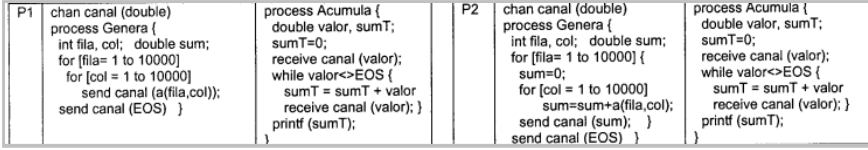
\includegraphics[]{assets/ejercicio-22.png}

\begin{enumerate}
\item ¿Qué hacen los programas?

\begin{answered}
Ambos programas realizan la suma de los elementos de una matriz. Aunque, difieren en el modo en que lo hacen.

En el \lstinline{Programa 1}: el proceso \lstinline{Genera} envía todos los valores al proceso \lstinline{Acumula}. El proceso \lstinline{Acumula} suma los valores que recibe desde \lstinline{Genera}.

En el \lstinline{Programa 2}: el proceso \lstinline{Genera} realiza la suma de los elementos de una fila y envia el resultado a \lstinline{Acumula}. El proceso \lstinline{Acumula}, recibe los resultados parciales y los adiciona en su acumulador.
\end{answered}


\item Analice desde el punto de vista del número de mensajes.

\begin{answered}
En el \lstinline{Programa 1}, el proceso \lstinline{Genera} envía todos los elementos de la matriz. Por lo cual, en esta solución, se están enviando $n*n = n^2$ mensajes.

En el \lstinline{Programa 2}, el proceso \lstinline{Genera} envía los valores acumulados de cada fila. Por lo cual, en esta solución, se están enviando $n$ mensajes.

\end{answered}

\item Analice desde el punto de vista de la granularidad de procesos.

\begin{answered}
El programa \lstinline{P2} tiene mayor granularidad, con respecto a \lstinline{P1}. Esto se debe a que, requiere menor comunicación (menos mensajes) para completar la tarea.
\end{answered}

\item ¿Cuál de los programas le parece el más adecuado para ejecutar sobre una arquitectura tipo cluster PCs? Justifique. 

\begin{answered}
Las arquitecturas cluster PC pueden ser catalogadas como grano grueso. Esto es, porque se componen de mucho procesadores; otorgando mayor potencia para cómputo. No obstante, tienen una menor performance en cuanto a comunicación.

Es deseable que la granularidad de la aplicación, se ajuste a la de la arquitectura. Para hacer un uso apropiado de los recursos y evitar rendimientos menores.

En este escenario, el programa, \lstinline{P1} parece el más adecuado para ejecutar en la arquitectura planteada.
\end{answered}
\end{enumerate}

%=======================================================================================================

\item Dado el siguiente bloque de código, indique para cada inciso qué valor queda en aux, o si el código queda bloqueado. Justifique su respuesta.

\begin{lstlisting}
aux = -1;
...
if (A == 0); P2?(aux) -> aux = aux + 2; # (1)
[] (A == 1); P3?(aux) -> aux = aux + 5; # (2)
[] (B == 0); P3?(aux) -> aux = aux + 7; # (3)
fi
\end{lstlisting}
\begin{enumerate}
\item Si el valor de A = 1 y B = 2 antes del if, y solo P2 envia el valor 6.
\begin{answered}
La guarda 1 queda bloqueada; su condición booleana es verdadera pero, su sentencia de comunicación generá bloqueo.
\end{answered}
\item Si el valor de A = 0 y B = 2 antes del if, y solo P2 envia el valor 8.
\begin{answered}
Solo la guarda 1 tiene éxito. Su sentencia guardada es ejecutada. El programa finaliza con \lstinline{aux = 10}.
\end{answered}
\item Si el valor de A = 2 y B = 0 antes del if, y solo P3 envia el valor 6.
\begin{answered}
Solo la guarda 3 tiene éxito. Su sentencia guardada es ejecutada. El programa finaliza con \lstinline{aux = 13}.
\end{answered}
\item Si el valor de A = 2 y B = 1 antes del if, y solo P3 envia el valor 9.
\begin{answered}
Todas las guardas fallan porque sus condiciones booleanas se evalúan como falsas. El programa finaliza con \lstinline{aux = -1}.
\end{answered}
\item Si el valor de A = 1 y B = 0 antes del if, y solo P3 envia el valor 14.
\begin{answered}
Las guardas 2 y 3, tienen éxito. Se elegirá una de las dos, de forma no deterministica y se ejecutará su sentencia guardada.

El programa finalizará con \lstinline{aux = 19 o 21}.
\end{answered}
\item Si el valor de A = 0 y B = 0 antes del if, P3 envia el valor 9 y P2 el valor 5.
\begin{answered}
Las guardas 1 y 3, tienen éxito. Se elegirá una de las dos, de forma no deterministica y se ejecutará su sentencia guardada.
    
El programa finalizará con \lstinline{aux = 16 o 7}.
\end{answered}
\end{enumerate}

%=======================================================================================================
\item ¿Qué significa el problema de interferencia en un programa concurrente? ¿Cómo puede evitarse? 
\begin{answered}
\emph{Apunte I: sección 1.4}
\end{answered}


%=======================================================================================================

\item Suponga que n2 procesos organizados en forma de grilla cuadrada. Cada proceso puede comunicarse solo con los vecinos izquierdo, derecho, de arriba y de abajo (los procesos de las esquinas tienen solo 2 vecinos, y los otros en los bordes de la grilla tienen 3 vecinos). Cada proceso tiene inicialmente un valor local v.
\begin{enumerate}
\item Escriba un algoritmo heartbeat que calcule el máximo y el mínimo de los n2 valores. Al terminar el programa, cada proceso debe conocer ambos valores.
\begin{answered}
La idea del algoritmo es que, cada proceso pueda propagar su valor hasta el proceso más lejano. La mayor distancia entre procesos, sin diagonales, está dada por $2(n-1)$ (esquina superior izquierda $\leftarrow \rightarrow$ esquina inferior derecha).
\end{answered}

\begin{lstlisting}
chan valores[1:n,1:n](int);

Process P[i=1..n;j=1..n]

int v;
int nuevo;
int min = v;
int max = v;
int rondas = 2(n-1);

for(k=1; k <= rondas; k++)

    foreach(vecinos => (x,y))
        send valores[x,y](v);

    foreach(vecinos => (x,y))
        receive valores[i,j](nuevo);
        if (nuevo < min) min = nuevo;
        if (nuevo > max) max = nuevo;
end;
end;
\end{lstlisting}


\item Analice la solución desde el punto de vista del número de mensajes.
\begin{answered}

{\renewcommand{\arraystretch}{2}%\
\begin{center}
\begin{tabular}{c c c c}
\textbf{Tipo} &  \textbf{Cantidad} & \textbf{Vecinos} & \textbf{Mensajes} \\
\hline
\textbf{Esquina} & 4 & 2 & $cantidad * vecinos * rondas$ \\
\hline
\textbf{Borde} & $4(n-2)$ & 3 & $cantidad * vecinos * rondas$ \\
\hline
\textbf{Internos} & $(n-2)^2$ & 4 & $cantidad * vecinos * rondas$\\
\end{tabular}
\end{center}}
\end{answered}

\item ¿Puede realizar alguna mejora para reducir el número de mensajes?
\begin{answered}
Podemos hacer que cada proceso, también, se comunique con sus diagonales. De esta forma; los procesos esquina tendrán 3 vecinos, los bordes 5 vecinos y el resto 8 vecinos.

Esto incrementará el número de mensajes enviados por cada proceso pero, también reducirá en la mitad la cantidad de rondas ($n-1$). Generando una reducción en la cantidad final de mensajes.

\begin{multicols}{2}
{\renewcommand{\arraystretch}{2}%\
\begin{center}
\begin{tabular}{c c c}
\textbf{Tipo} &  \textbf{Cantidad} & \textbf{Vecinos} \\
\hline
\textbf{Esquina} & 4 & 3 \\
\hline
\textbf{Borde} & $4(n-2)$ & 5 \\
\hline
\textbf{Internos} & $(n-2)^2$ & 8 \\
\end{tabular}
\end{center}}  
\columnbreak
{\renewcommand{\arraystretch}{2}%\
\begin{center}
\begin{tabular}{c c c}
\textbf{n} &  \textbf{Sin Diagonales} & \textbf{Con Diagonales} \\
\hline
4 & 288 & 252\\
\hline
6 & 1200 &  1100\\
\hline
8 & 3136 &  2940\\
\end{tabular}
\end{center}}  
\end{multicols}

\end{answered}

\item Indique que mecanismo de pasaje de mensajes utilizaría. Justifique.

\begin{answered}
En mi opinión, utilizaría PMA. Particularmente, porque su primitiva \lstinline{send} no es bloqueante. Esto nos evita demoras innecesarias al momento de propagar el valor de un proceso, en particular con $n$ muy grandes.    
\end{answered}


\end{enumerate}

%=============================================================================================

\item En los protocolos de acceso a sección crítica vistos en clase, cada proceso ejecuta el mismo algoritmo. Una manera alternativa de resolver el problema es usando un proceso coordinador. En este caso, cuando cada
proceso SC[i] quiere entrar a su sección crítica le avisa al coordinador, y espera a que éste le de permiso. Al
terminar de ejecutar su sección crítica, el proceso SC[i] le avisa al coordinador.
Desarrolle protocolos para los procesos SC[i] y el coordinador usando sólo variables compartidas (no
tenga en cuenta la propiedad de eventual entrada).

\begin{lstlisting}[multicols=2]
int request[n] = ([n] 0),
    grant[n] = ([n] 0);

Process Worker[i = 1..n]
    
# Seccion no critica ...

request[i] = 1;
while(grant[i] == 0) skip;
# Seccion Critica
grant[i] = 0;
# Seccion no critica ...
end;

Process Coordinator
while (true)
    for (j = 1; j < n; j++)
        if (request[j] == 1)
            request[j] = 0;
            grant[j] = 1;
            while (grant[j] == 1) skip;
        end;
    end;
end;
end;
\end{lstlisting}

%====================================================================

\item Suponga que la solución a un problema es paralelizada sobre p procesadores de dos maneras diferentes.
En un caso, el speedup (S) está regido por la función S=p-1 y en el otro por la función S=p/2. ¿Cuál de las
dos soluciones se comportará más eficientemente al crecer la cantidad de procesadores? Justifique
claramente.
\begin{answered}
    \emph{Apunte IV: sección 1.4 (Escalabilidad)}
\end{answered}

%=====================================================================

\item Analice que tipos de mecanismos de pasaje de mensajes son más adecuados para resolver problemas del tipo Cliente-Servidor, Pares que interactúan, filtro y productores- consumidores. Justificar.

\begin{answered}
En los problemas del tipo \textbf{pares que interactúan, filtros y productores/consumidores}; el esquema de \textbf{comunicación entre procesos}, por lo general, es \textbf{unidireccional}. Un proceso, envía un mensaje a otro y no requiere una respuesta, del receptor de dicho mensaje, para continuar con su trabajo.

Dado este escenario, descripto en el párrafo anterior, la opción más adecuada es la de utilizar \textbf{pasaje de mensajes asincrónico}. Ya que su primitiva \lstinline{send} no es bloqueante para el emisor; permitiendole despachar su mensaje y continúar con su trabajo.

En los problemas del tipo \textbf{cliente/servidor}; el esquema de \textbf{comunicación entre procesos} es \textbf{bidireccional}. Un proceso, cliente, envía una solicitud a un proceso servidor; y espera por la respuesta correspondiente.

Dado este escenario, descripto en el párrafo anterior, la opción más adecuada es la de utilizar \textbf{pasaje de mensajes sincrónico}. Ya que su primitiva \lstinline{send} es bloqueante para el emisor; impidiendo que continue con su ejecución hasta obtener la respuesta correspondiente.

Además, en los problemas del tipo \textbf{cliente/servidor}, tenemos que tener en cuenta la \textbf{cantidad de canales a definir}. Esto supone un problema ya que; necesitamos al menos un canal para que el servidor reciba solicitudes y tantos canales, de respuesta, como procesos clientes tengamos. 

Existen técnicas que resuelven esta problematica, sobre la cantidad de canales a definir. Una de ellas es \textbf{Rendezvous} y otra \textbf{Remote Procedure Call (RPC)}.
\end{answered}
\end{QandA}
\end{document}